\chapter{Anforderungen und Analyse}\label{kap:anforderunganalyse}

\section{Ziel der Arbeit}\label{sec:zielderarbeit}


Wie in der Einleitung \ref{kap:einleitung} beschrieben, soll 
ein CNN Basiertes System zur Wildtiererkennung entwickelt 
werden, das für dir Inferenz den Neural Compute Stick 2 verwendet.
Dabei sollte neben der reinen Erkennung auch eine Lokalisierung 
der erkannten Tiere im Bild stattfinden. Gängige Techniken dafür 
werden im nächsten Abschnitt erläutert.
\\
Dabei soll das Deep Learing Modell im Rahmen der gegebenen 
möglichkeiten und Limitierungen der Hardware möglichst 
genau und Robust sein, sodass es auch für die graustufen 
Bilder der Infrarot Kamera zuverlässig funktioniert.
Da eine erhöht Genauigkeit auch immer mit einer größeren
Latenz für der Inferenzzeit einhergeht war dies ein mit 
zu berücksichtigender Punkt.
\\
Neben training und evaluierung eines geeigneten Deep Learning Modells,
war die Implementierung der Anwendung, welche die Inferenz 
des Modells ausführt ein weiterer Bestandteil der Arbeit.
\\
Diese soll voll autonom auf dem Raspberry Pi laufen,
über eine mobile Netzwerk Verbindung verfügen und 
mittels eines geeigneten Kommunikations Protokolls die 
die erkannten und abgespeicherten Bilder an einen
Heim Pc senden.
Des weiteren sollte eine geeignete Kamera verwendet werden, die 
sowohl normale, als auch Infrarot Aufnahmen machen kann.


\section{Related Work}\label{sec:related_work}

% papers
% SSD: \cite{liuSSDSingleShot2016}
% speed/acc: \cite{huangSpeedAccuracyTradeOffs2017}
% blogpost: \cite{wengObjectDetectionPart2018}

% Bilder:
% SSD: \cite{SSDSingleShot}
% speed acc: \cite{huangSpeedAccuracyTradeOffs2017}

Wie in \ref{subsec:objdet_det} erwähnt, werden für die 
Object Detection neben einem CNN zur Feature extaction 
weiteere strukturen/framework benötigt zur lokalisierung 
des Objekts im Bild

Die entwicklung immer genauerer und effizienterer 
Frameworks ist Gegenstand aktueller Forschung und lassen 
sich wie in dem übersichtspaper \cite{ouaknineReviewDeepLearning}
beschrieben in die zwei grundarten \textit{Region proposal based} 
und den \textit{Regression/Classification Based} einteilen.



\subsection{Faster R-CNN}
Region Proposial Based Ansatz, \dots \cite{renFasterRCNNRealTime2016a}
bei dem das RPN ein Bild als unput erhällt und
daraus mögliche regionen für objekte im Bild findet.

hier in einem Fully Convolutional realisiert, über dessen 
Feature Maps im Sliding winow verfahren vordefinierte Anker
 Boxen konvoliert werden. Der Resultieruende Vektor wird 
 dann in einen binären FC Layer (cls) zur klassifizierung und 
einen box-regressor layer (reg) für die Koordinaten gegeben.


\begin{figure}[H]
    \centering
    \label{fig:faster_rcnn}
    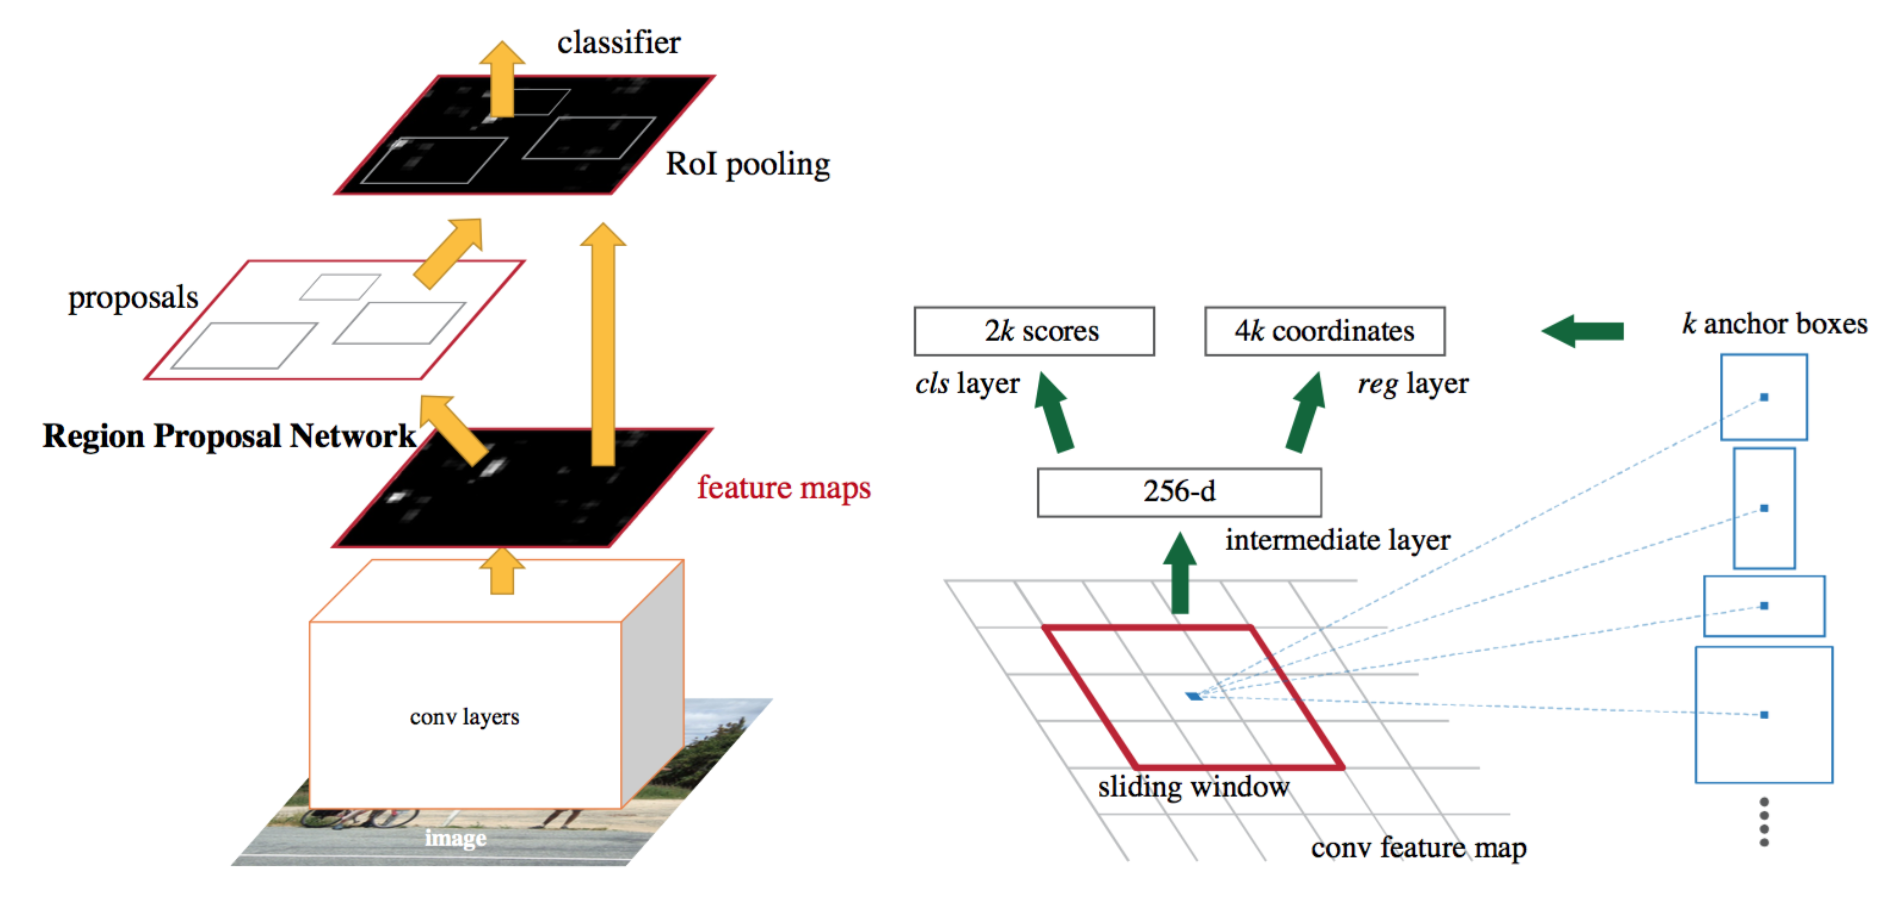
\includegraphics[width=0.7\textwidth]{faster-RCNN_architecture.png}
    \caption{Faster R-CNN, quelle: \cite{ObjectDetectionDummies2017b}}
\end{figure}



\subsection{SSD: Single Shot MultiBox Detector}
Ist ein Regression/Classification Based Ansatz ... \cite{liuSSDSingleShot2016}

Dabei werden dem Backbone CNN wetere feature Layer verschiedener größe 
angehänget, welche zusammen mit default anker boxen und einem score 
für die anwesenheit des objakts in der box in einen non max supression 
layer gegeben, welcher die finalen predictions bestimmt.


\begin{figure}[H]
    \centering
    \label{fig:faster_rcnn}
    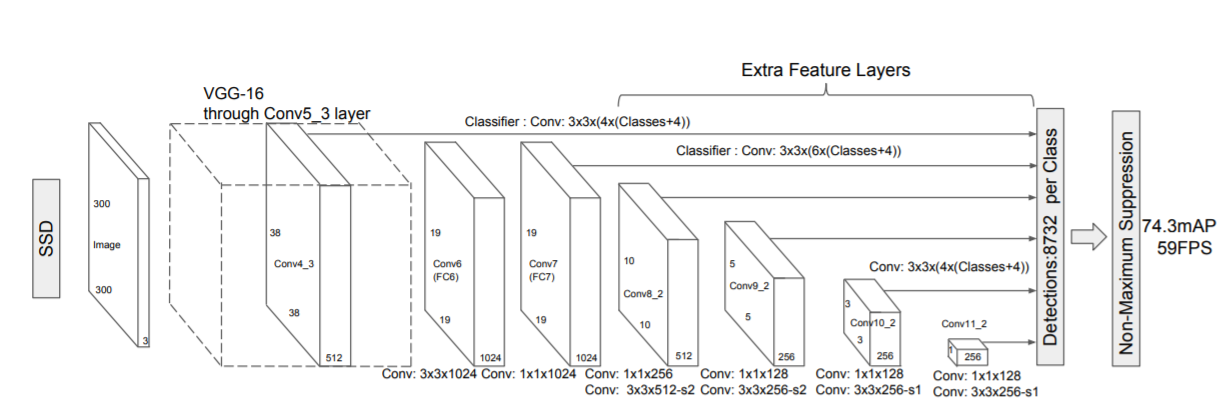
\includegraphics[width=0.7\textwidth]{ssd_architecture.png}
    \caption{SSD, quelle: \cite{SSDSingleShot}}
\end{figure}

